Dieses Experiment dient zur Veranschaulichung der dynamischen Prioritäten. Diese Situation kann, dezentral, nämlich nicht durch feste Prioritäten gelöst werden.

\textbf{Aufbau des Experiments}
\begin{figure}[H]
    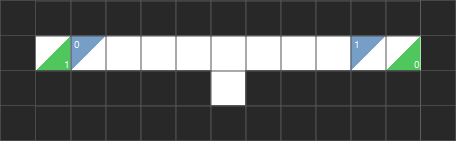
\includegraphics[height=32mm]{images/tunnel_turnout.png}
    \centering
    \caption{Aufbau für die Vorbeifahrt zweier Agenten in einem Tunnel mit einer kleinen Ausweichbucht}
    \label{fig:ausweichbucht}
\end{figure}
Zwei sich gegenüberstehende Agenten versuchen, in einer elf Felder langen und ein Feld schmalen Engstelle aneinander vorbei auf ihre Zielpositionen zu fahren. Der Tunnel hat in der Mitte ein zusätzliches freies Feld, das von den Agenten genutzt werden muss, um aneinander vorbei zu fahren.

\textbf{Erwartete Beobachtungen}\newline
Zuerst werden die beiden Agenten aufeinander zu fahren. Dann wird einer der beiden Agenten zurückgedrängt werden. Wenn der zurückgedrängte Agent sich nicht weiter zurückdrängen lässt, wird dieser seine Priorität erhöhen und den zu erst drängenden Agenten in die Ausweichbucht drängen, was dann beiden Agenten ermöglicht aneinander vorbei zu ihren Zielpositionen zu fahren. Es kann auch passieren, dass ein Agent die Ausweichbucht direkt anfährt und es zu keiner Verdrängung kommt.